\begin{problem}{Where is my ICP?}{standard input}{standard output}{1 second}{256 megabytes}

\begin{center}
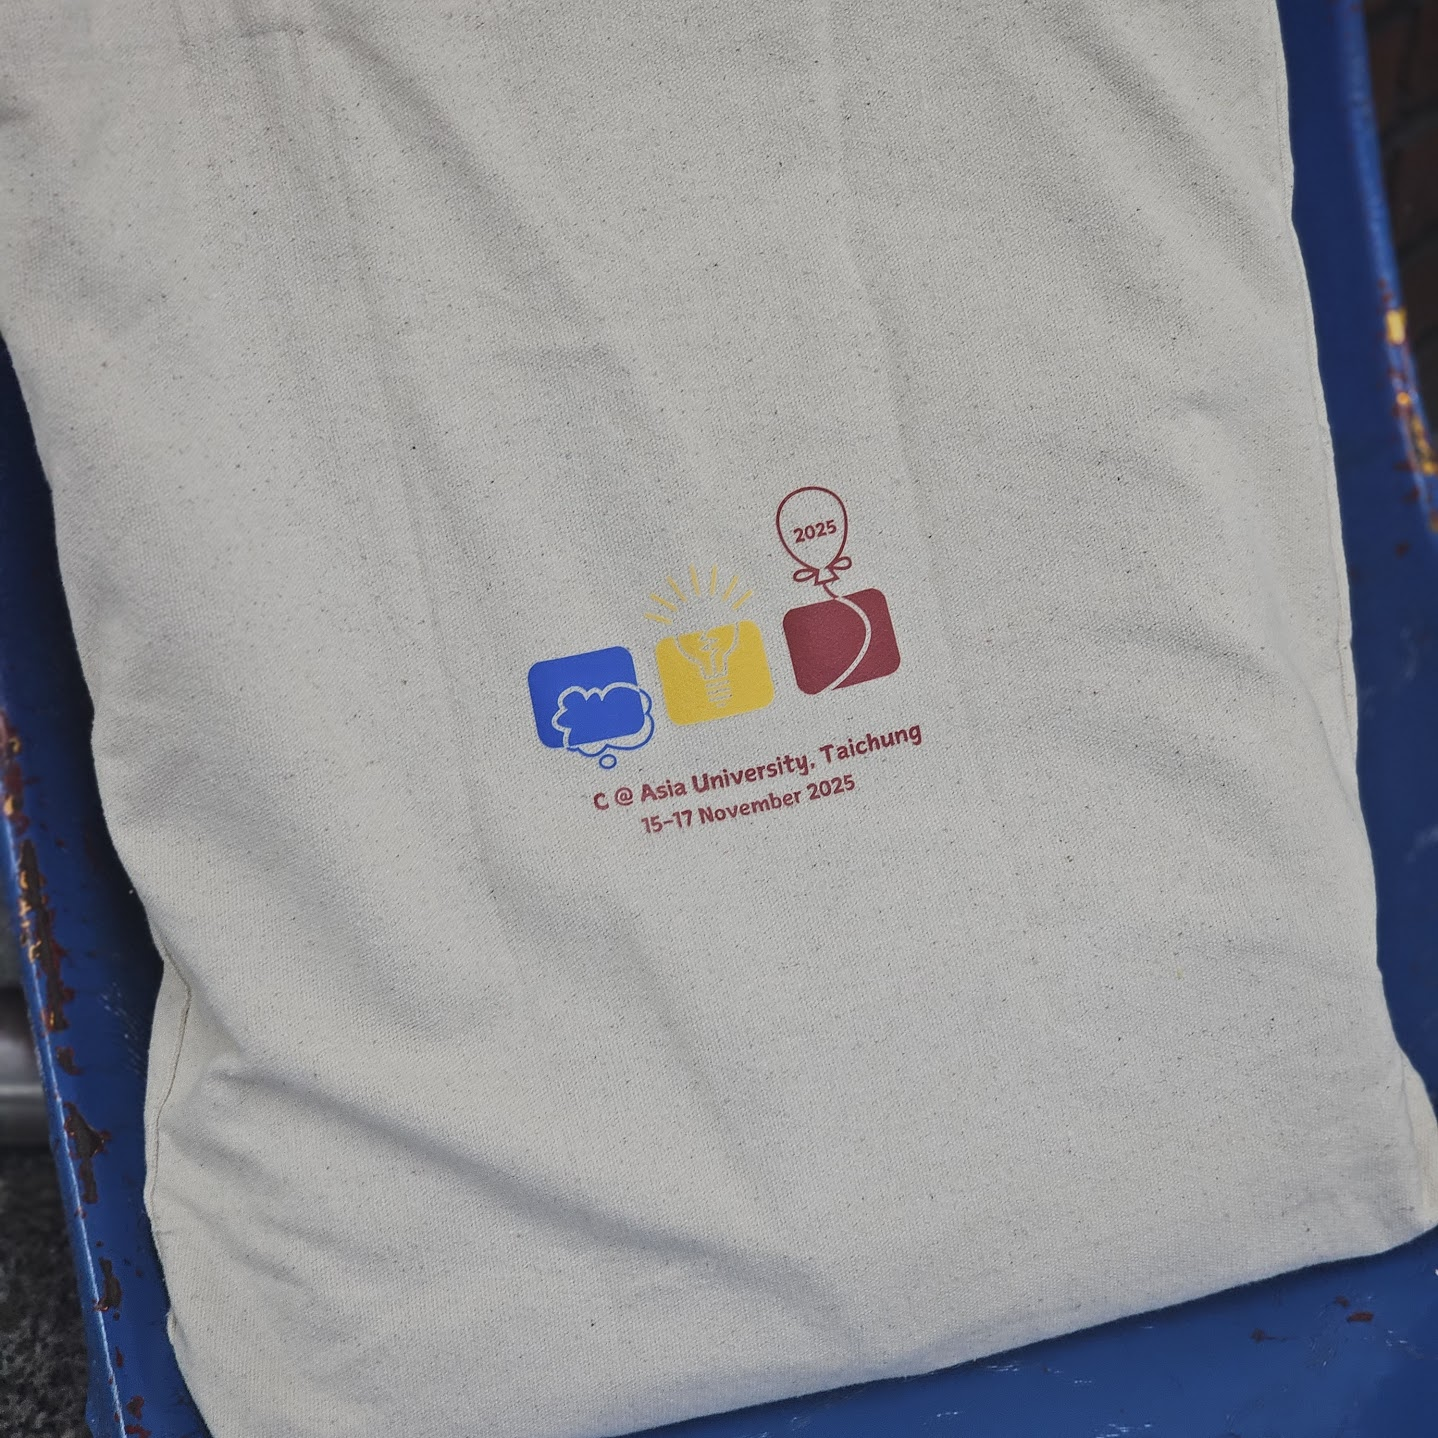
\includegraphics[width=15cm]{icpc.jpg}
\end{center}


민성이는 2025년 ICPC 대만 리저널에 참여하고 받은 에코백을 보며 슬퍼하고 있다. 

원래 에코백에는 \texttt{ICPC} 네 글자가 멋지게 인쇄되어 있었지만, 몇 글자가 떨어져 나가고 문자열 $S$만 남았기 때문이다.

슬퍼하는 민성이를 위해, 창민이는 지난 SCON 운영진이 남겨 둔 문자 스티커 $T$의 일부를 사용해 잃어버린 글자를 채워 가방에 다시 \texttt{ICPC} 문자열을 만들어 주려 한다. 

문자열 $S$와 $T$가 주어졌을 때, 창민이가 민성이의 가방에 \texttt{ICPC} 문자열을 복원할 수 있는지 판별하라.


\InputFile

첫째 줄에 가방에 남아 있는 문자열 $S$의 길이 $N$이 주어진다. ($1 \le N \le 4$)

둘째 줄에 문자열 $S$가 주어진다. $S$는 `I`, `C`, `P`로만 구성되며, ``ICPC``에서 순서를 유지한 채 일부 문자가 사라진 문자열이다.

셋째 줄에 문자 스티커 $T$의 길이 $M$이 주어진다. ($1 \le M \le 100$)

넷째 줄에 문자열 $T$가 주어진다. $T$는 대문자 알파벳으로만 구성되며, 같은 알파벳이 여러 번 등장할 수 있다.

\OutputFile
$T$에 포함된 스티커를 사용하여 ``ICPC``를 복원할 수 있으면 ``m4us happy``를, 그렇지 않으면 ``m4us sad``를 출력한다.

\Examples

\begin{example}
\exmpfile{example.01}{example.01.a}%
\exmpfile{example.02}{example.02.a}%
\end{example}

\Note
지문과 달리 실제로 창민이는 민성이를 놀렸고, 그 때문인지 2026 Asia Pacific Championship에 가서 받은 가방에 붙어있던 스티커가 떨어졌다. 

주의: 문자열을 저장하기 위해 char 배열을 사용하는 경우, 문자열의 끝을 나타내는 널 문자('\0')를 저장할 공간이 추가로 필요하다. 예를 들어 길이가 100인 문자열을 저장하려면 배열의 크기를 최소 101 이상으로 선언해야 안전하다.

\end{problem}

